Al ya tener definido el algortimo se Shor, se comenzo a desarrollar un programa que funcione para cualquier número dado usando la libreria
de Qiskit (código \ref{cod:shorquanrum}). Este fue subido a la plataforma \href{https://quantum-computing.ibm.com/}{\textit{IBM Q Experience}} con un formato de 
Jupyter Notebook, ya que este es el que recibe para poder ejecutar el código. Se creo otro código el cual sigue los lineamientos del algoritmo de criba general del cuerpo de números.
(codigo \ref{cod:time_clasic}), los dos códigos generan archivos de texto que contienen el tiempo de procesamiento de cada algoritmo.
\begin{table}[H]
    \centering
    \begin{tabular}{|c|c|c|c|c|} \hline
        Algortimo & Número a factorizar & IBM Device & Lanzamientos & Repeticiones \\ \hline 
        CCGN & \multirow{3}{*}{21} & - & -& \multirow{3}{*}{1000}\\  \cline{1-1} \cline{3-4}
        Shor (Local) &  & \multirow{2}{*}{Vigo}& \multirow{2}{*}{1000}& \\ \cline{1-1}
        Shor (IBM Q) &  & &  &\\\hline
    \end{tabular}
    \caption{Parámetros de entrada de cada algoritmo de factorización.}
    \label{table:parametros}
\end{table}
Usando los parámetros de entrada de la tabla \ref{table:parametros} en cada algoritmo de los códigos \ref{cod:shorquanrum} y \ref{cod:time_clasic} se obtuvieron los tiempos de procesamiento y al estar
factorizando el mismo número repetidas veces se pueden obtener los tiempos promedios en los cuales se tarda cada algoritmo en su diferente situación. Estos resultados son los mostrados en la tabla \ref{tabla:resultados}.
\begin{table}[H]
    \centering
    \begin{tabular}{ccc} \hline
        Algoritmo & Promedio (ms) & $\sigma$ (ms ) \\ \hline
        Clasico & 0.056 & 0.0096 \\
        Shor &0.036& 0.0153 \\
        Shor IBM &0.024 &0.0102 \\ \hline
    \end{tabular}
    \caption{Promedio y desviación estandar de cada algoritmo de factotización ejecutados en una computadora clásica y cuántica.}
    \label{tabla:resultados}
\end{table}
\begin{figure}[H]
    \centering
    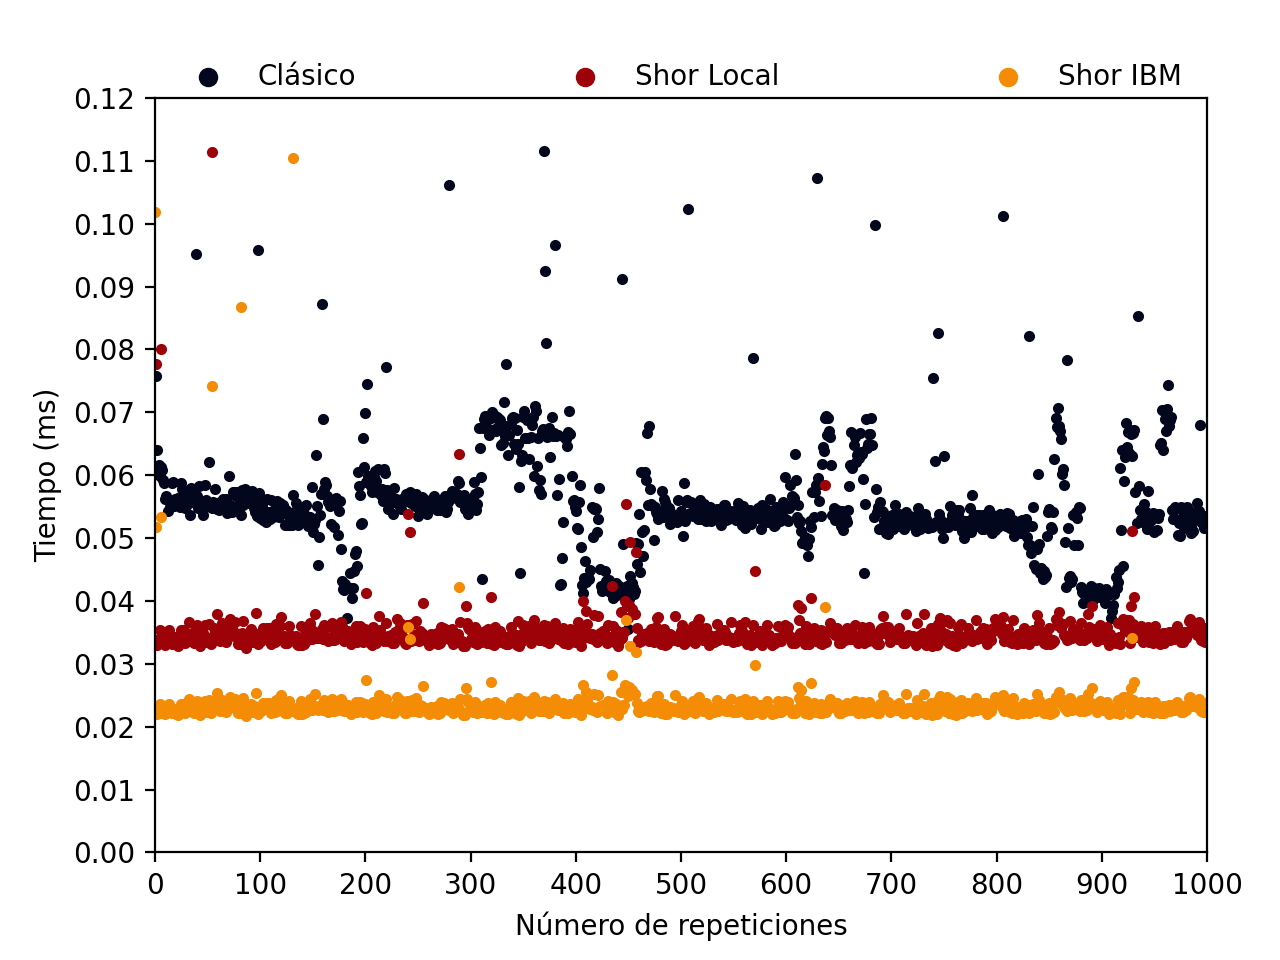
\includegraphics[scale=0.7]{images/time.png}
    \caption{Comparación de los tiempos de procesamiento de los códigos \ref{cod:shorquanrum} y \ref{cod:time_clasic}, el código \ref{cod:shorquanrum} fue 
    ejecutado en una computadora clásica y en una computadora cuántica.}
    \label{fig:time}
\end{figure}
Con estos mismos resultados se genero la figura \ref{fig:time}, en donde se muestra el tiempo de procesamiento de cada algoritmo en cada repetición que se realizó.